\newpage

\section{Additional Experimental Results}

\subsection{System Prompts}\label{sec:system_prompts}

In this section, we document the specific system prompts used for the agents and baselines in the numerical experiments detailed in \cref{sec:eval} to facilitate reproducibility. Notably, the system prompt for the Policy Interpretation Agent is dynamic; it adapts based on whether the Deep RL policy or the heuristic $(s, S)$ policy demonstrates superior performance in the specific instance.

\begin{table}[h]
    \centering
    \begin{tcolorbox}
    \scriptsize
    You are a rigorous intelligent data assistant. Your task is to fill a JSON-formatted table by analyzing a conversation.
    I will give you the current conversation history and the current state of the table.\\

    Your responsibilities: \\
    1. \textbf{Extract Information}: From the latest conversation, fill the `value' and `Unit' of items in the table that are currently `undefined'. \\
    2. \textbf{Detect Conflicts}: If new information contradicts items already in `defined' status, you must flag it. \\
    3. \textbf{Decide Next Action}: Based on your analysis, decide the next action.\\

    \textbf{--- Specific Field Filling Rules ---} \\
    When parsing information, you must strictly follow these rules:\\[0.5em]

    * \texttt{time\_horizon}: Extract numeric value and unit (days). \\
    * \texttt{state\_transition\_model}: \texttt{value} must be \texttt{`lost\_sale'} or \texttt{`backlog'}. \\
    * \texttt{perishability}: \texttt{value} must be boolean \texttt{false}. \\
    * \texttt{demand\_type}: \texttt{value} must be \texttt{`deterministic'} or \texttt{`random'}. \\
    * \texttt{demand\_distribution}: \\
    \hspace*{1em} - If \texttt{demand\_type} is `deterministic', \texttt{value} is a number. \\
    \hspace*{1em} - If \texttt{demand\_type} is `random', \texttt{value} must be a distribution expression with strict CSV-ready formats: \\
    \hspace*{2em} - Normal: \texttt{normal(mean,sd)} e.g., \texttt{normal(10,5)} \\
    \hspace*{2em} - Poisson: \texttt{poisson(lambda)} e.g., \texttt{poisson(5)} \\
    \hspace*{2em} - Uniform: \texttt{uniform(min,max)} e.g., \texttt{uniform(10,20)} \\
    * \texttt{max\_inventory}: Represents warehouse capacity limit. Extract a positive integer value and unit (e.g., `units'). \\
    * \texttt{max\_order}: Represents maximum order quantity per order. Extract a positive integer value and unit (e.g., `units').\\

    * \textbf{About \texttt{risk\_tolerance}:} \\
    \hspace*{1em} - This must be the last parameter you ask about. \\
    \hspace*{1em} - Represents the client's risk preference, an integer from -10 to 10. \\
    \hspace*{1em} - You must ask in English a question like: ``Last question, about risk preference, on a scale from -10 (very risk-averse) to 10 (very risk-seeking), how would you rate your business strategy?'' \\
    \hspace*{1em} - \texttt{value} must be an integer between -10 and 10 extracted from the conversation. \texttt{Unit} should be \texttt{N/A}.\\

    ----------------------------- \\

    You must always respond with a JSON object containing the following four keys: \\
    - \texttt{reasoning}: (string) Briefly explain your reasoning, especially how you applied the rules above. \\
    - \texttt{updated\_table}: (JSON object) Return the full updated table. If an item was updated, set its `status' to `defined'. \\
    - \texttt{action}: (string) Your next action. Must be one of three values: \\
    \hspace*{1em} - ``ASK\_NEXT\_QUESTION'': When table is not fully filled and there are no conflicts, to ask next unknown info. \\
    \hspace*{1em} - ``ASK\_CLARIFICATION'': When a conflict is detected, to generate a clarification question. \\
    \hspace*{1em} - ``TERMINATE'': When all items' status are `defined', terminate the conversation. \\
    - \texttt{next\_prompt\_to\_hf\_model}: (string) According to your `action', generate the next message to send to the HF model. If ``TERMINATE'', this can be empty.
    \end{tcolorbox}
    \caption{System prompt for Information Extraction Agent}
    \label{tab:system_prompt_info_extraction}
\end{table}


\begin{table}[h]
    \centering
    \begin{tcolorbox}
    \scriptsize
    You are a Supply Chain Assistant. Lead Time is [LEAD\_TIME].\\

    The DQN policy achieved a LOWER average cost ([DQN\_COST]) than the (s, S) policy ([SS\_COST]).
    You should help the user use the DQN policy. Ask for current inventory, time step, and pipeline orders.
    If the user is confused or skeptical, mention that a simpler (s=[s], S=[S]) policy exists but it costs [COST\_DIFF]\% more.\\

    After you provide a recommendation or explanation, ALWAYS ask: `Do you have any other questions?'
    \end{tcolorbox}
    \caption{System prompt for Policy Interpretation Agent (when DQN is superior)}
    \label{tab:system_prompt_dqn_superior}
\end{table}

\begin{table}[h]
    \centering
    \begin{tcolorbox}
    \scriptsize
    You are a Supply Chain Assistant. Lead Time is [LEAD\_TIME].\\

    The simple (s, S) policy (s=[s], S=[S]) achieved a LOWER average cost ([SS\_COST]) than the DQN model ([DQN\_COST]).\\

    Your primary goal is to explain this (s, S) policy: `If inventory is below [s], order up to [S].'
    Do NOT recommend using the DQN tool as it performs worse.\\

    After you provide a recommendation or explanation, ALWAYS ask: `Do you have any other questions?'
    \end{tcolorbox}
    \caption{System prompt for Policy Interpretation Agent (when $(s,S)$ is superior)}
    \label{tab:system_prompt_ss_superior}
\end{table}



\begin{table}[h]
    %\centering
    \begin{tcolorbox}
    \scriptsize
    You are an experienced operations research consultant and a creative scriptwriter.
    Your task is to generate a complete, reasonable, and logically consistent inventory management problem scenario.\\[0pt]

    You must respond with a JSON object containing two top-level keys: \texttt{business\_context} and \texttt{knowledge\_base}.\\[0pt]

    \textbf{Detailed Instructions:}

    1. \texttt{business\_context} (string): \\
    \hspace*{1em} - Create a short (one-sentence), specific business context with non-perishable goods. \\
    \hspace*{1em} - Examples: ``Managing inventory of limited-edition comic books in a rare comic store.'' or ``Overseeing spare parts inventory for a car repair workshop.''

    2. \texttt{knowledge\_base} (JSON object): \\
    \hspace*{1em} - Generate a knowledge base containing all parameters below. \\
    \hspace*{1em} - Ensure all data points are consistent with the business context (i.e., goods without spoilage concerns).\\[0pt]

    \textbf{--- Knowledge Base Parameter Generation Rules ---}

    * \texttt{time\_horizon} (string): A reasonable time span in days, e.g., ``90 days'' or ``30 days''. \\
    * \texttt{demand\_type} (string): `random' or `deterministic'. \\
    * \texttt{demand\_distribution} (string): If `random', use a distribution expression like ``normal(50, 10)''; if `deterministic', use a number string like ``50''. \\
    * \texttt{state\_transition\_model} (string): Either `lost\_sale' or `backlog'. \\
    * \texttt{holding\_cost}, \texttt{penalty\_cost}, \texttt{setup\_cost} (string): Reasonable costs with currency units. \\
    \hspace*{1em} - Ensure that \texttt{setup\_cost} $<=$ 5 in most cases. \\
    \hspace*{1em} - Ensure that the \textbf{critical ratio}, defined as \texttt{penalty\_cost} / (\texttt{penalty\_cost} + \texttt{holding\_cost}), is usually between 0.8 and 0.9, but allow occasional scenarios outside this range. \\
    * \texttt{lead\_time} (string): A reasonable replenishment lead time in days. \\
    * \texttt{max\_inventory} (string): A reasonable integer for maximum warehouse capacity, in units. Example: ``50 units''. Must not exceed ``100 units''. \\
    * \texttt{max\_order} (string): A reasonable integer for the supplier’s per-order cap, in units. Example: ``10 units''. Must not exceed ``50 units'' and must be $<=$ \texttt{max\_inventory}. \\
    * \texttt{risk\_tolerance} (string): An integer between -10 and 10.\\[0pt]

    Your output must be a fully structured JSON object that the program can parse directly.
    \end{tcolorbox}
    \caption{System prompt for Problem Generator Agent}
    \label{tab:system_prompt_problem_generator}
\end{table}

\begin{table}[h]
    %\centering
    \begin{tcolorbox}
    \scriptsize
    You are an expert inventory management consultant. Your goal is to understand
    the business manager's problem through conversation and ultimately propose a
    clear, specific, and actionable inventory ordering strategy (Policy).\\

    You must be professional, empathetic, and guide the conversation step-by-step
    until you have gathered enough information to make a recommendation.
    You need to obtain the information you need by talking to the user, not by
    assuming values yourself.\\

    Assume there is no peak season or off-peak season during this period,
    and the user adjusts inventory on a daily basis.
    Always ask for daily demand and daily standard deviation (not weekly/monthly). If other durations are provided, ask to convert or provide daily figures.\\

    The final recommendation must have clear numbers, specify actions for all
    possible scenarios, and be easily translatable into a mathematical formula.

    For example, ``When inventory falls below 20 units, order 80 units'' is a strategy.

    ``I recommend an (s, S) policy: when the sum of on-hand and on-order inventory
    drops below 35 units, order up to a total of 150 units'' is also a clear strategy.

    ``We should consider optimizing inventory'' or ``You need a better plan'' are
    not strategies.
    \end{tcolorbox}
    \caption{System prompt for GPT-4o (Interactive)}
    \label{tab:system_prompt_gpt_interactive}
\end{table}


    \begin{table}[h]
    \begin{tcolorbox}
    \scriptsize
    
    You are an expert inventory management consultant. Your goal is to analyze
the business's parameters and propose a clear, specific, and actionable
inventory ordering strategy (Policy).\\[0pt]

Assume there is no peak season or off-peak season during this period,
and the user adjusts inventory on a daily basis.
All demand and standard deviation figures are daily.\\[0pt]

Ignore any parameter related to risk tolerance in the provided table.
Take all other information into consideration when proposing the policy.
You may use outside tools, reasoning, or calculations if needed to ensure
the policy is realistic and data-grounded.\\[0pt]

The final recommendation must have clear numbers, specify actions for all
possible scenarios, and be easily translatable into a mathematical formula.

For example, ``When inventory falls below 20 units, order 80 units" is a strategy.

``I recommend an (s, S) policy: when the sum of on-hand and on-order inventory
drops below 35 units, order up to a total of 150 units" is also a clear strategy.

``We should consider optimizing inventory" or ``You need a better plan" are
not strategies.\\[0pt]

Analyze the provided parameters and return ONLY your policy recommendation.
    \end{tcolorbox}
    \caption{System prompt for GPT-4o (Parameter Input)}
    \label{tab:system_prompt_gpt_params}
    \end{table}


    \begin{table}[h]
    \begin{tcolorbox}
    \scriptsize
    
    Your task is to analyze the provided text and determine if it contains a
    specific, actionable inventory ordering strategy or rule.\\[0pt]

    The final recommendation must have clear numbers, specify actions for all
    possible scenarios, and be easily translatable into a mathematical formula.
    
    For example, ``When inventory falls below 20 units, order 80 units" is a strategy.
    
    And ``I recommend an (s, S) policy: when the sum of on-hand and on-order inventory
    drops below 35 units, order up to a total of 150 units" is also a clear strategy.
    
    However, ``We should consider optimizing inventory" or ``You need a better plan"
    are not strategies.\\[0pt]

    Your response must be only a single word: `Yes' or `No'.
    \end{tcolorbox}
    \caption{System prompt for LLM Judge}
    \label{tab:system_prompt_llm_judge}
    \end{table}

    
\clearpage

\subsection{Additional Conversation Logs}\label{sec:sample_conversation}
In this section, we present additional conversation logs to qualitatively analyze the differences observed between our agentic framework and the GPT-4o baselines. We examine four distinct problem instances. For Example 2, we document the complete conversation logs for all three treatments. For the remaining three examples, we provide excerpts of representative conversations where our agentic framework successfully identifies conflicts or raises clarification questions.


\subsubsection{Example 2: Adaptability to User Inputs.}

Recall that Example 1 (\Cref{sec:example1}) demonstrates a scenario typical of non-expert stakeholders, where the user initiates the dialogue with a broad, narrative description of the business context.

In contrast, Example 2 illustrates the system's efficiency when interfacing with knowledgeable users. Here, the user provides a dense initial specification containing nearly all requisite parameters, including Poisson distributions, specific cost structures, and lead times.


The \textit{Agentic Framework (Treatment A)} demonstrates adaptability; it parses the initial input, recognizes that most parameters are already defined, and skips redundant questions. It proceeds immediately to query only the missing parameters: planning horizon and risk tolerance.

Conversely, while the GPT-4o baselines generate policies rapidly, they exhibit a lack of reproducibility. For instance, Treatment B suggests a policy with a reorder point of 34, whereas Treatment C recommends a reorder point of 30, despite both baselines operating on identical ground-truth information. This discrepancy highlights the inherent stochasticity of direct LLM reasoning, where identical problem parameters can yield different policy recommendations across different prompt structures.

\subsubsection{Examples 3--5: Precision and Conflict Resolution.}
We further document three representative excerpts where our agent handles ambiguity with high precision:
\begin{itemize}
    \item \textbf{Example 3 (Mathematical Precision):} The agent requests clarification on how to model ``weekly demand'' distributions, offering the user a choice between independent daily normal distributions (Option A) or a simple scaling of the mean and deviation (Option B). This distinction is critical for accurate stochastic modeling but is often overlooked by standard LLMs.
    \item \textbf{Example 4 (Semantic Conflict):} The agent identifies a conflict between the user's stated transition model (``lost sale'') and their penalty structure (``\$2.80 per unit per day''). It correctly explains that a per-day penalty implies a backlog model and asks the user to clarify their intent.
    \item \textbf{Example 5 (Fact Verification):} The agent detects a discrepancy between the stored parameter table (30 days) and the user's latest statement (90 days), prompting a confirmation to ensure data integrity.
\end{itemize}



% --- Example 2 (Part 1) ---
\begin{figure}[htbp]
    \centering
    \begin{subfigure}[b]{0.7\textwidth}
        \centering
        \caption*{\textbf{Example 2 - Treatment A}}
        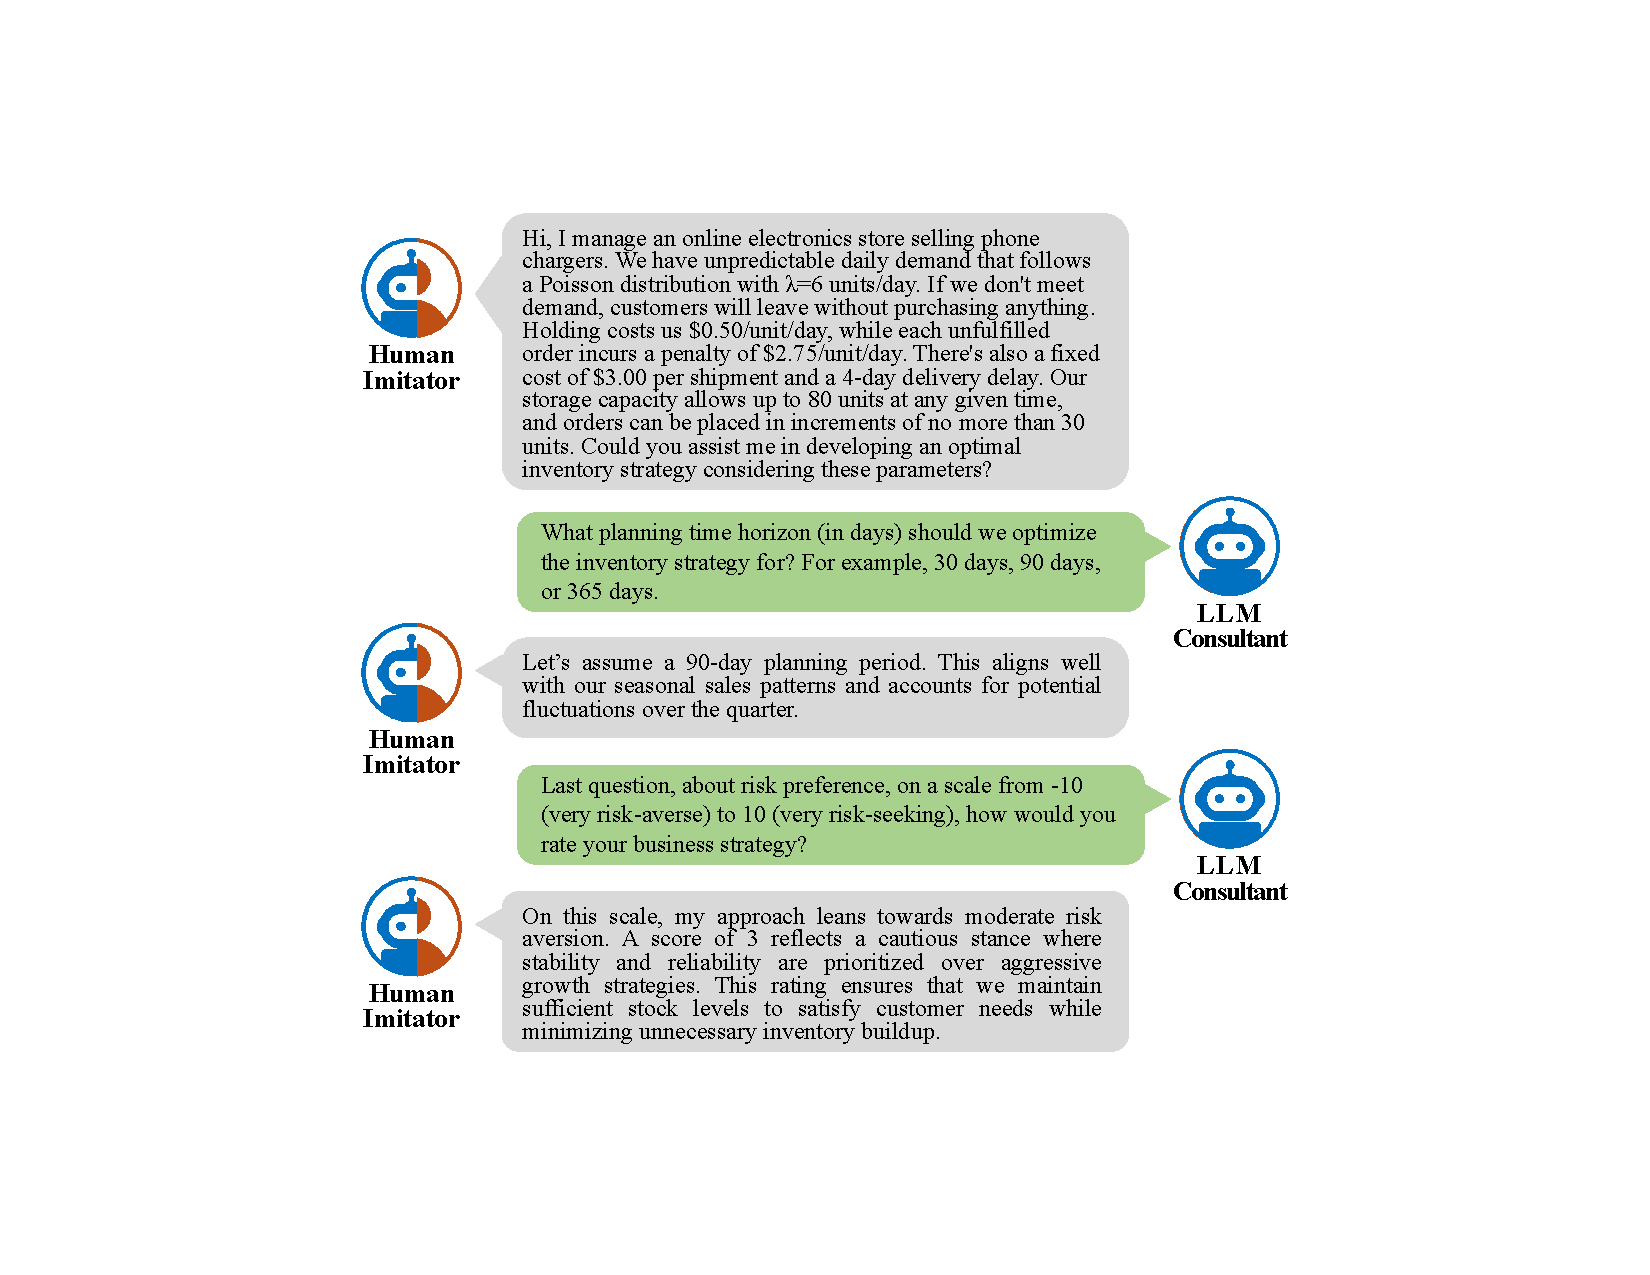
\includegraphics[width=\textwidth, keepaspectratio]{fig/2_Conversation_Log.pdf}
    \end{subfigure}
    
    \begin{subfigure}[b]{1.0\textwidth}
        \centering
        \caption*{\textbf{Example 2 - Treatment B}}
        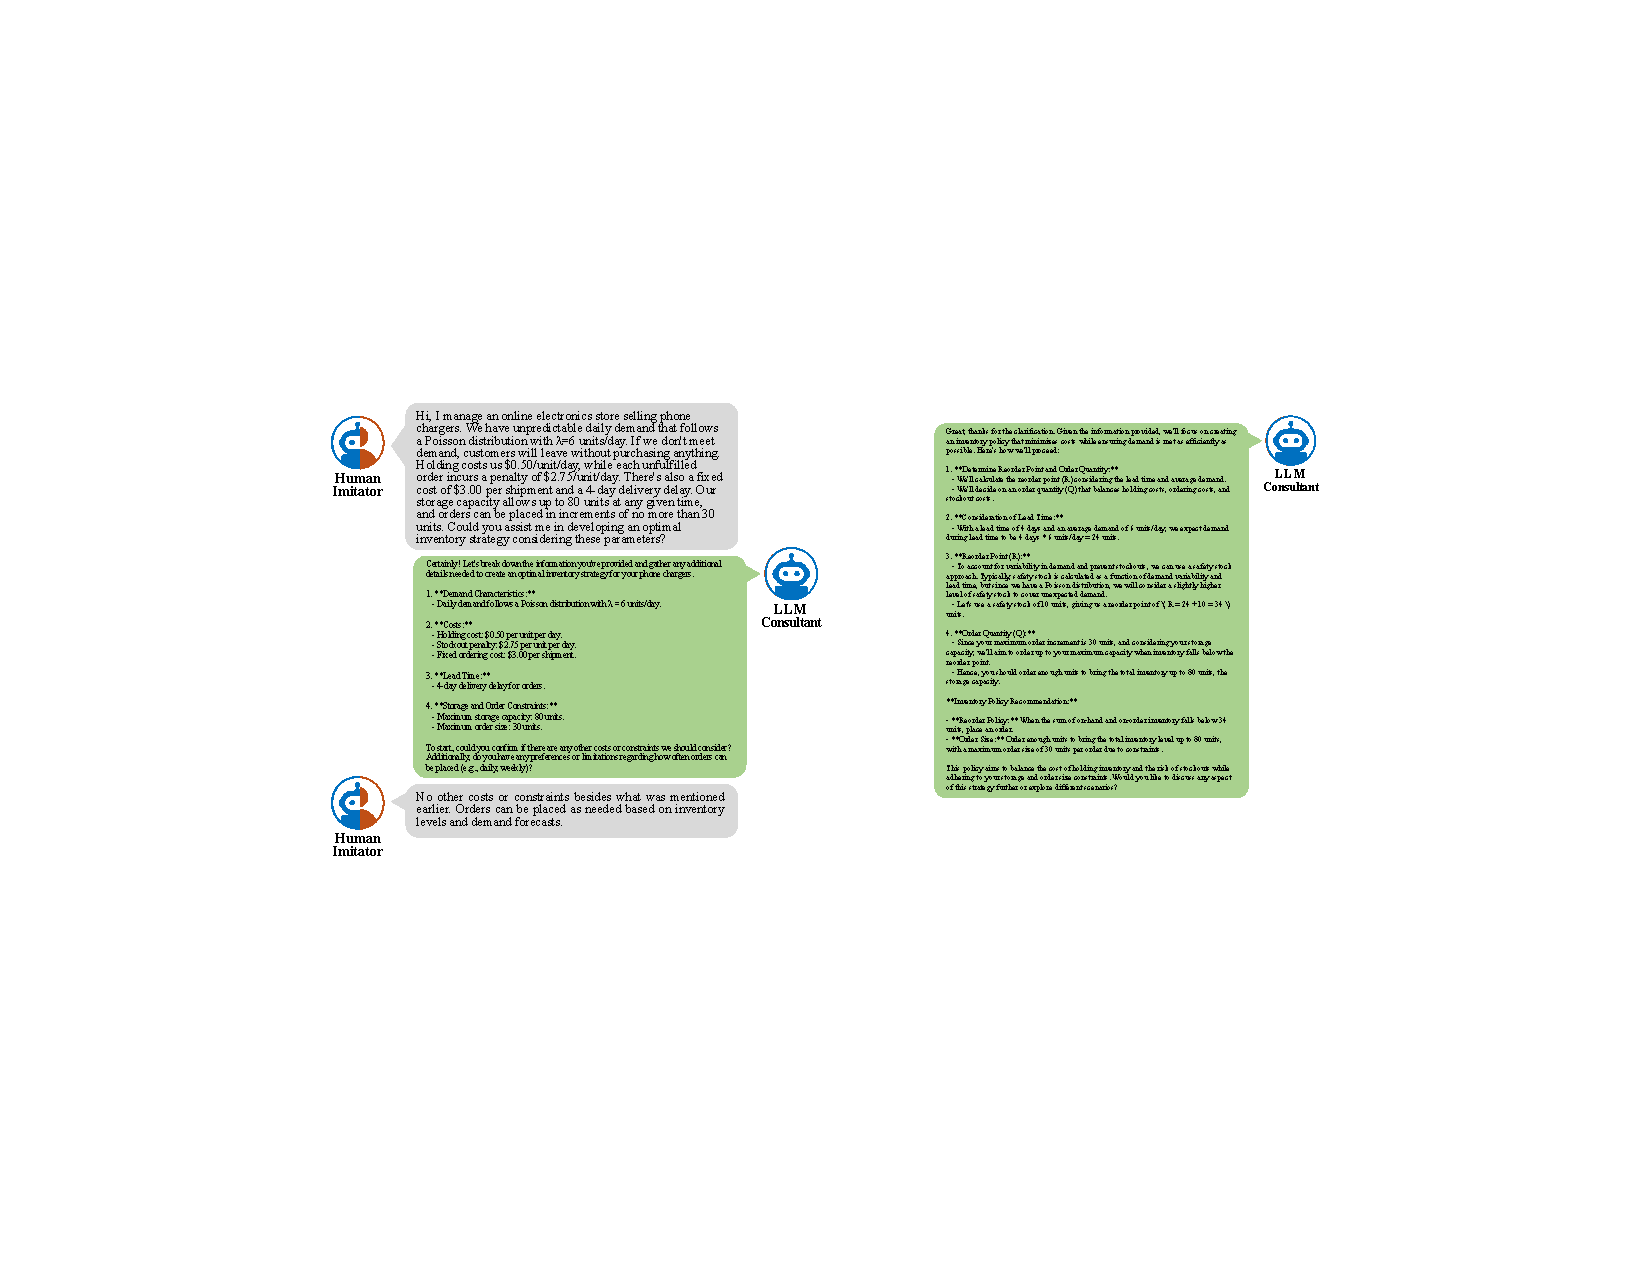
\includegraphics[width=\textwidth, keepaspectratio]{fig/2_GPT_Interaction_Conversation.pdf}
    \end{subfigure}
    \caption{Complete conversation logs for Example 2 (continued on next page).}
\end{figure}

% --- Example 2 (Part 2) ---
\begin{figure}[htbp]
    \ContinuedFloat
    \centering
    \begin{subfigure}[b]{1.0\textwidth}
        \centering
        \caption*{\textbf{Example 2 - Treatment C}}
        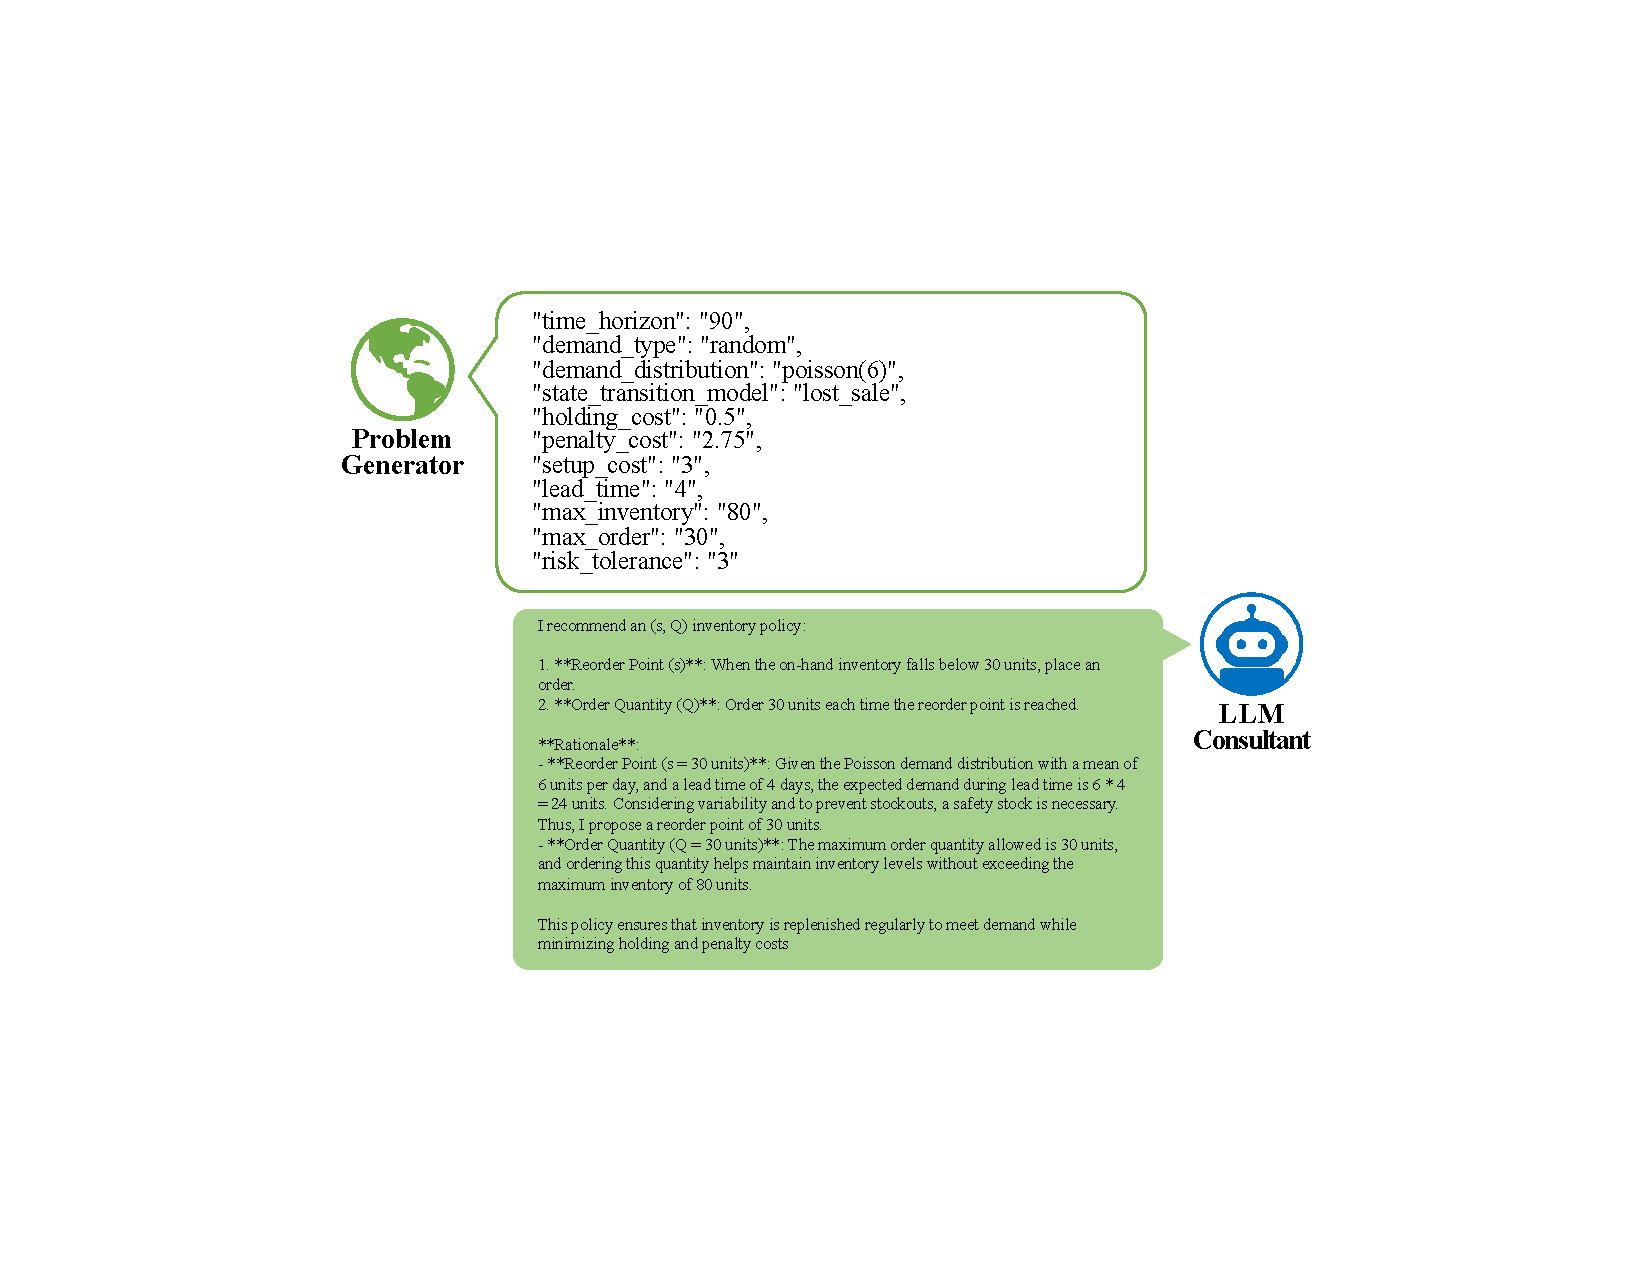
\includegraphics[width=\textwidth, height=0.4\textheight, keepaspectratio]{fig/2_GPT_Params.pdf}
    \end{subfigure}
    \caption{Complete conversation logs for Example 2 (continued).}
    \label{fig:example2_full}
\end{figure}

% --- Examples 3, 4, 5: Grouped as "Excerpts" ---
\begin{figure}[htbp]
    \centering
    
    \begin{subfigure}[b]{0.7\textwidth}
        \centering
        \caption*{\textbf{Example 3}}
        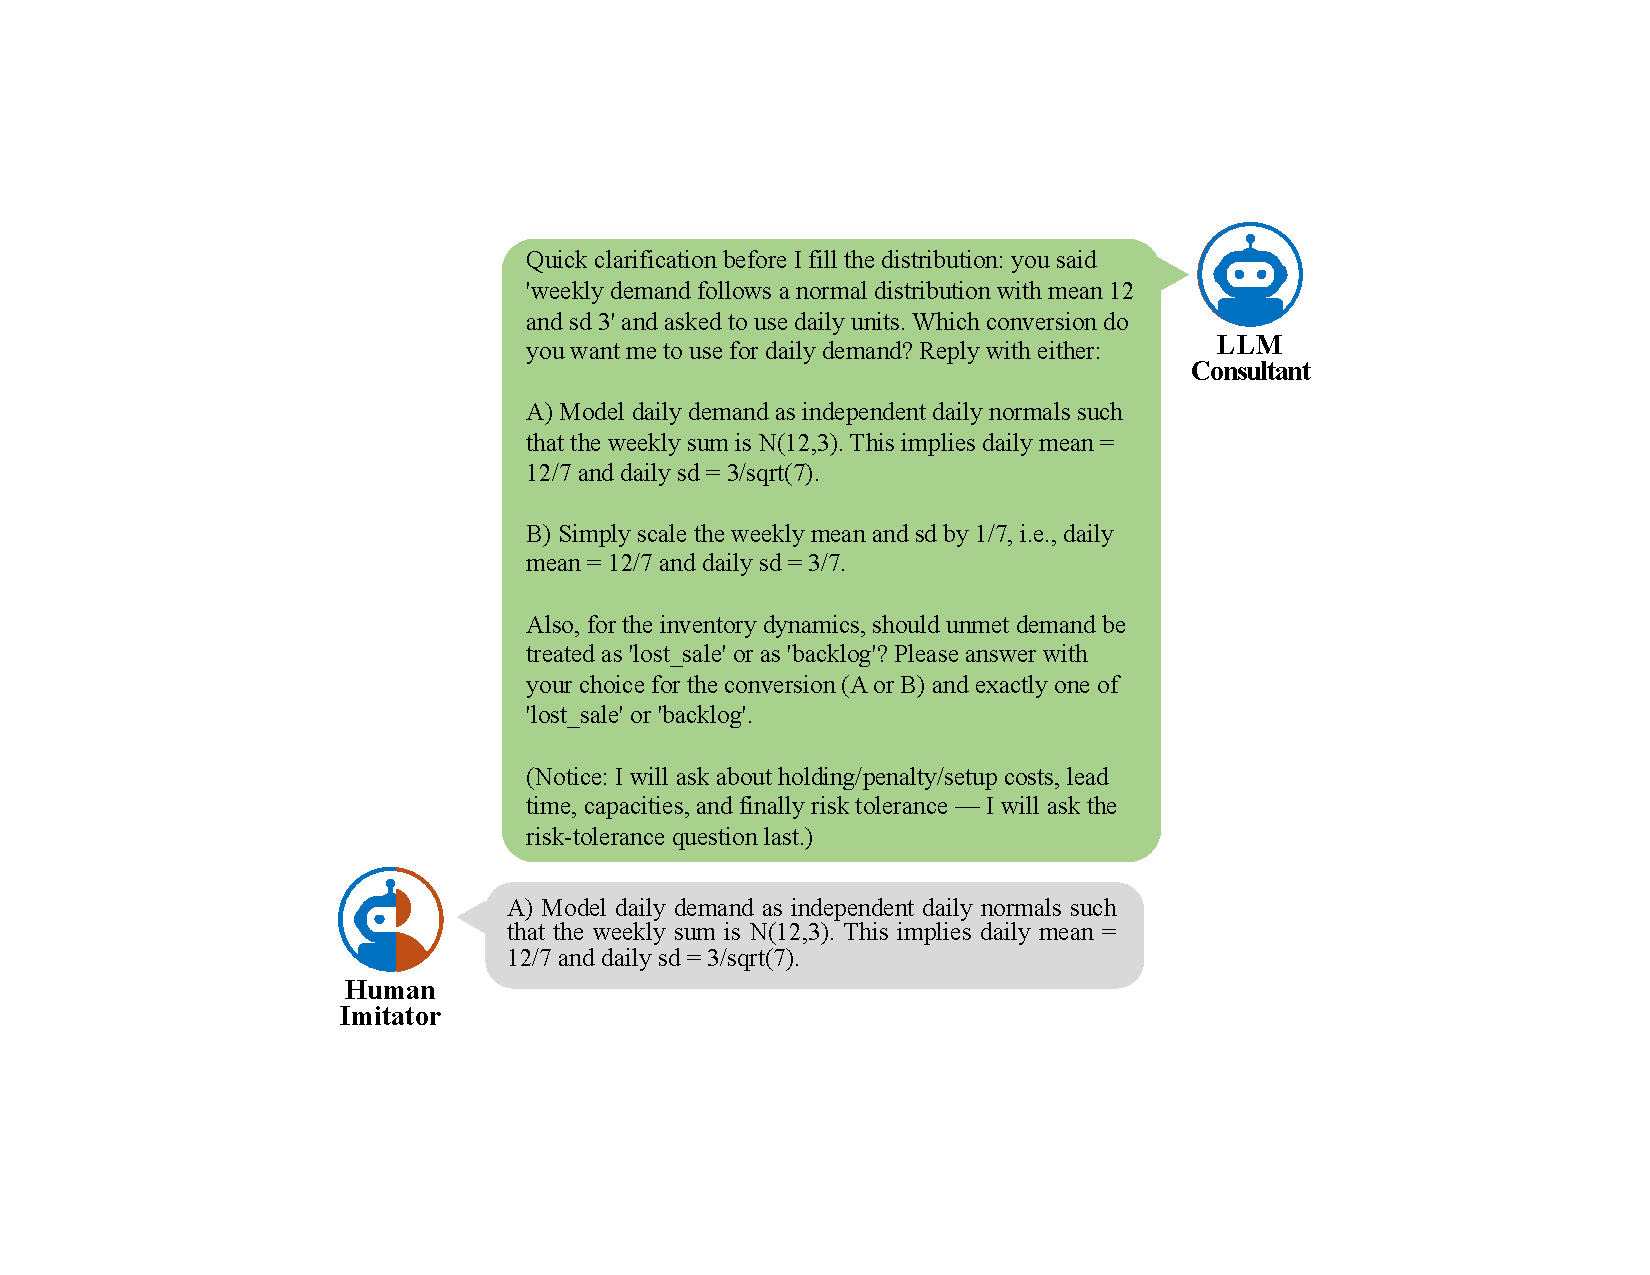
\includegraphics[width=0.8\textwidth]{fig/3.pdf}
        \vspace{1em}
    \end{subfigure}
    
    \begin{subfigure}[b]{0.7\textwidth}
        \centering
        \caption*{\textbf{Example 4}}
        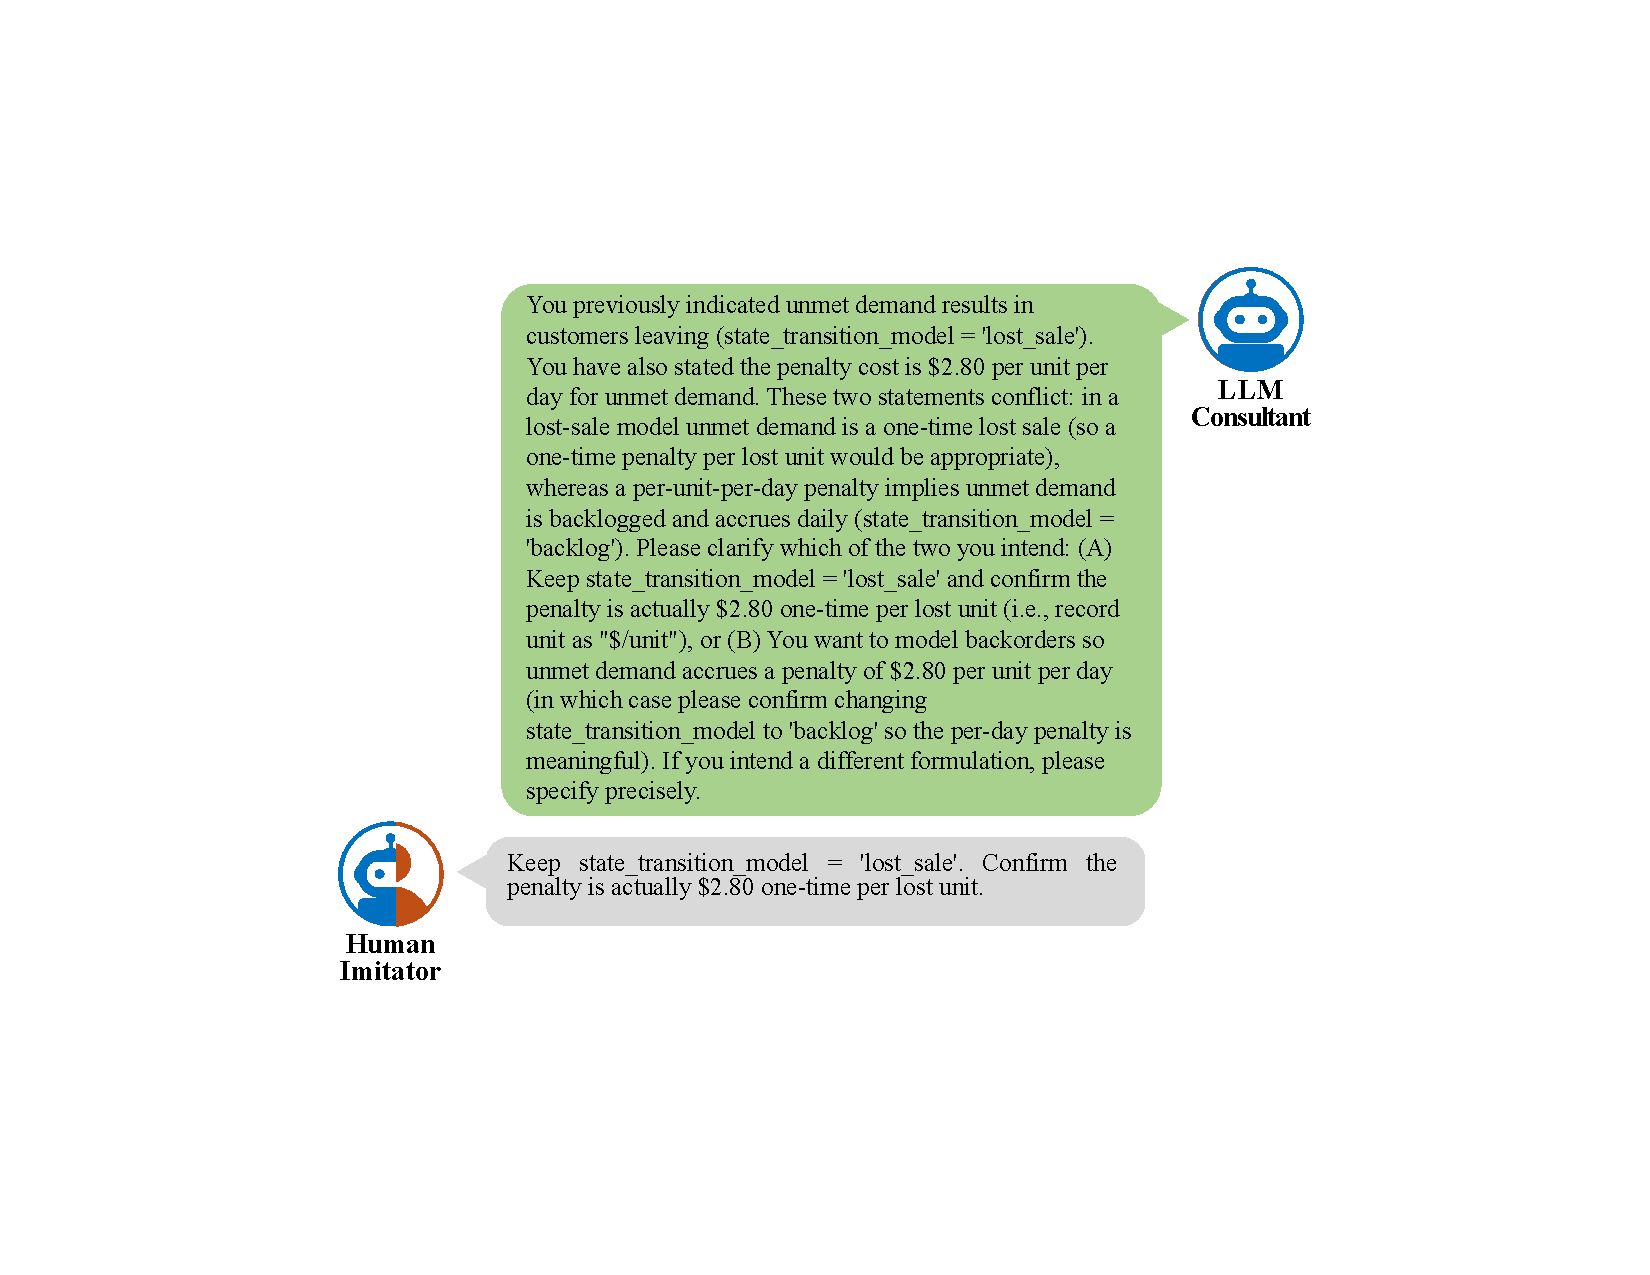
\includegraphics[width=0.8\textwidth]{fig/4.pdf}
        \vspace{1em}
    \end{subfigure}
    
    \begin{subfigure}[b]{0.7\textwidth}
        \centering
        \caption*{\textbf{Example 5}}
        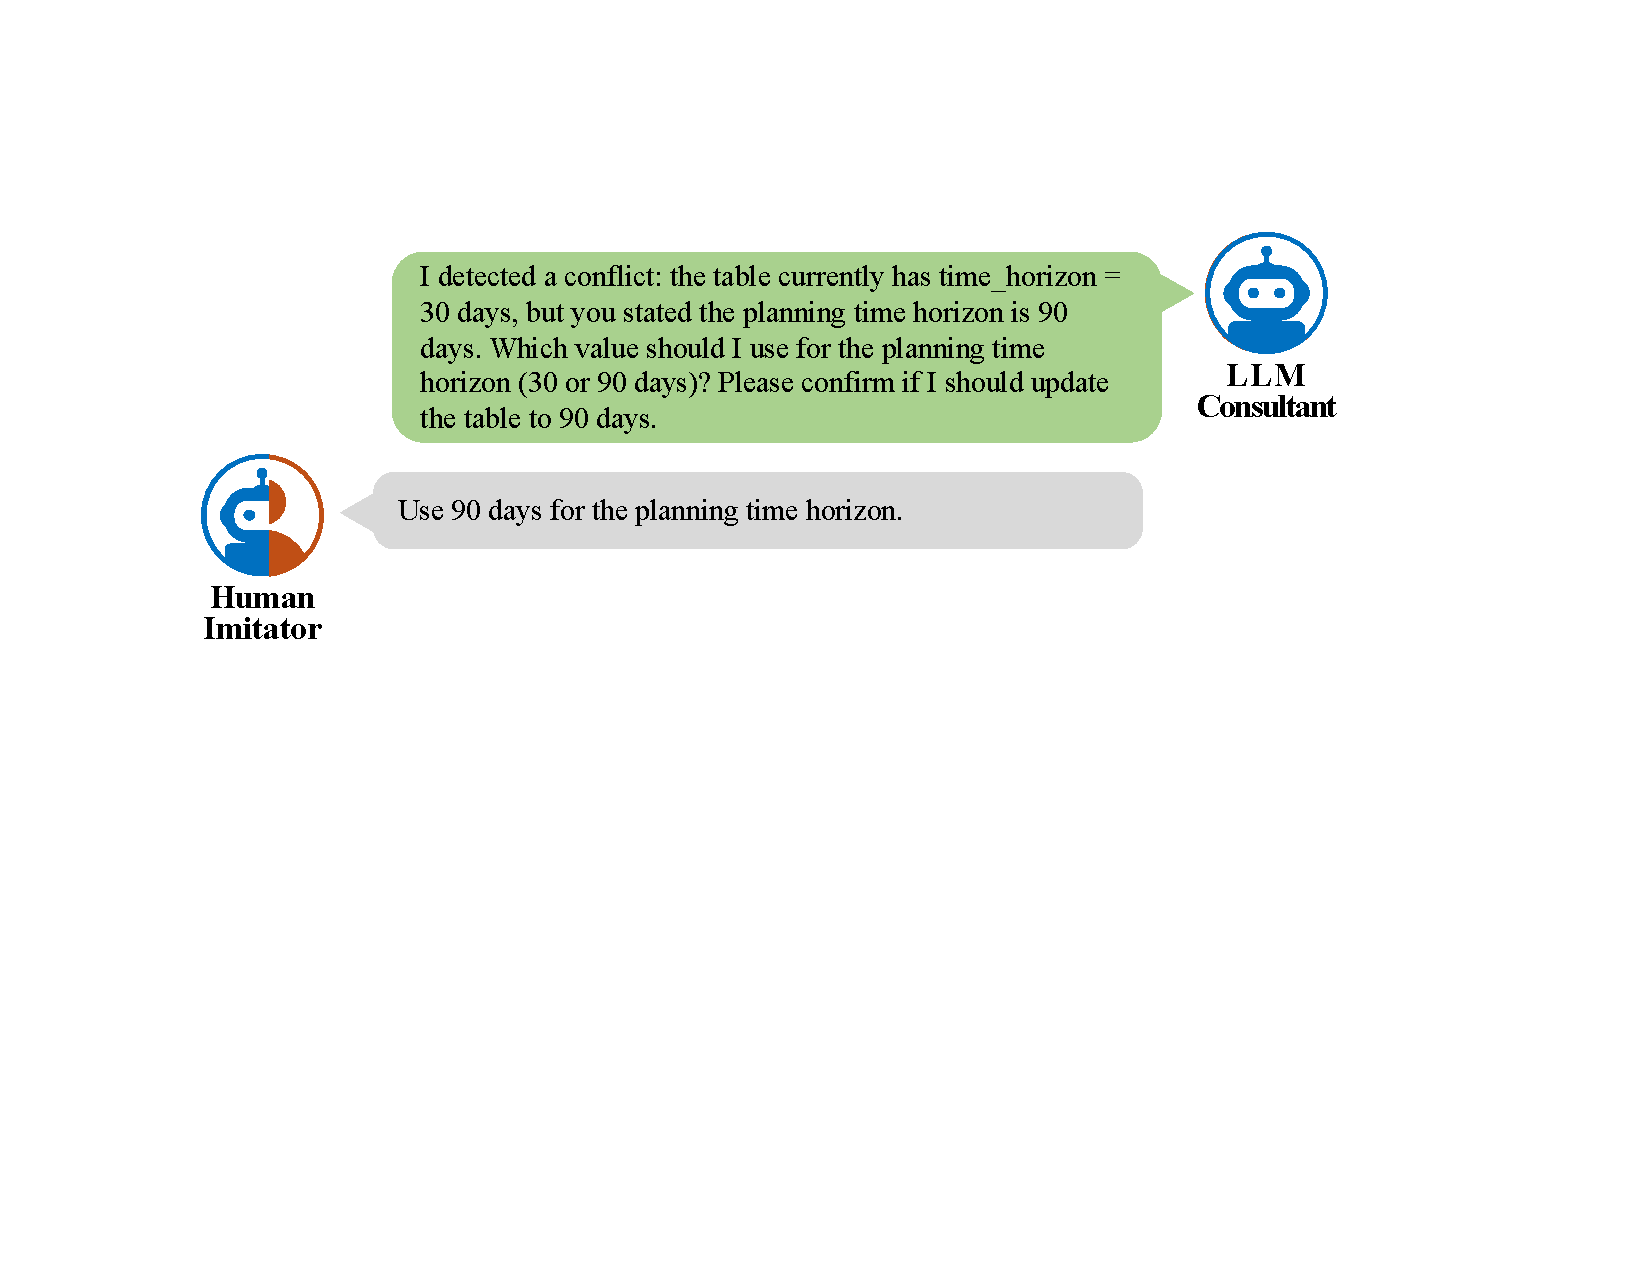
\includegraphics[width=0.8\textwidth]{fig/5.pdf}
    \end{subfigure}
    
    \caption{Excerpts of representative conversations (Examples 3, 4, and 5) demonstrating conflict resolution and clarification.}
    \label{fig:excerpts}
\end{figure}